\documentclass[10pt]{beamer}

\ifx\pdftexversion\undefined
\usepackage[dvips]{graphicx}
\else
%\usepackage[pdftex]{graphicx}
\DeclareGraphicsRule{*}{mps}{*}{}
\fi

\usepackage[english]{babel}
\usepackage[T1]{fontenc}
\usepackage[utf8]{inputenc}
\usepackage{amsmath}
\usepackage{bbold}
\usepackage[french]{algorithm2e}
\usepackage{multimedia}
\usepackage{tikz}

\definecolor{dark-green}{rgb}{0.2,0.8,0.2}
\useoutertheme{infolines}

\usetheme{Berlin}
\usecolortheme{dolphin}
\beamertemplatenavigationsymbolsempty
\addtobeamertemplate{navigation symbols}{}{%
    \usebeamerfont{footline}%
    \usebeamercolor[fg]{footline}%
    \hspace{1em}%
    \normalsize
    \insertframenumber/\inserttotalframenumber
}

\newcommand{\beginbackup}{
   \newcounter{framenumbervorappendix}
   \setcounter{framenumbervorappendix}{\value{framenumber}}
}
\newcommand{\backupend}{
   \addtocounter{framenumbervorappendix}{-\value{framenumber}}
   \addtocounter{framenumber}{\value{framenumbervorappendix}} 
}

\setbeamercovered{transparent} 

\title{State set representation for hybrid system reachability analysis}
\author[Owen Rouillé]{Owen Rouillé\\[0.3cm]
\footnotesize
Supervised by \textbf{Erika Ábrahám} and \textbf{Stefan Schupp}
}

%\titlegraphic{
%\scalebox{0.4}{
%    		\includegraphics[scale=0.10]{images/LogoENS.eps} \hspace{1.0cm}
%    		\includegraphics[scale=0.6]{images/LogoUnivRennes1.pdf} \hspace{0.5cm}
%        	\includegraphics[scale=0.35]{images/LogoInria.eps} \hspace{0.5cm}
%        	\includegraphics[scale=0.65]{images/LogoHybrid.eps}
%        }
%}

\begin{document}
\maketitle

%trucs qui clignottent(minipage?)
%enumeration ; ; ; . . .
%\cdot


\section{Introduction}
\subsection{Hybrid systems}
\begin{frame}{What is an hybrid system?}
\begin{center}
\vspace*{-1.5cm}
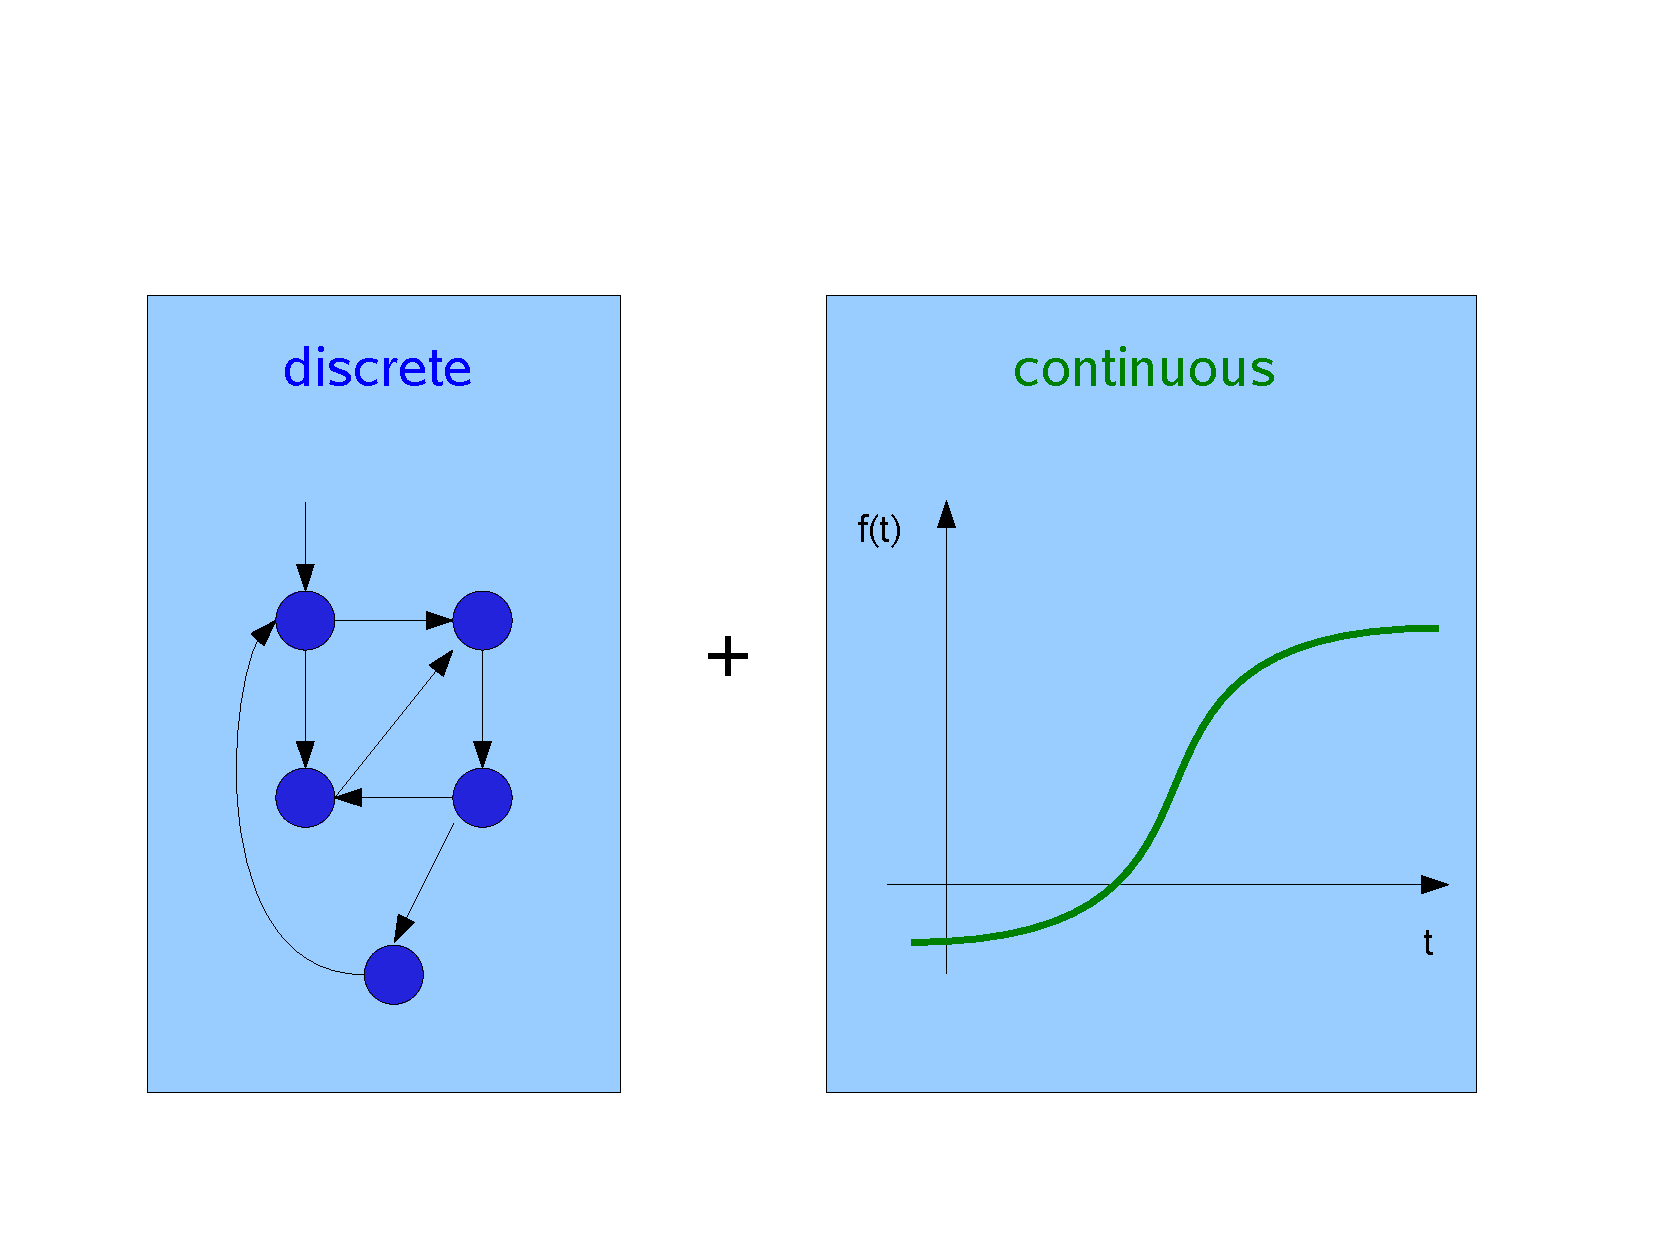
\includegraphics[width=\columnwidth]{images/cs.pdf}
%ajouter photos?
\end{center}
\end{frame}

\begin{frame}{A model: the hybrid automaton}
\begin{center}
\begin{columns}[c]
\begin{column}{5cm}
\hspace*{-0.5cm}
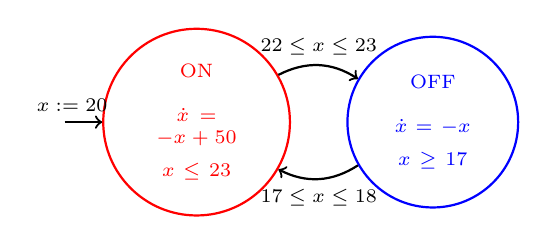
\begin{tikzpicture}[scale=0.6]
  \node[draw, circle, text width = 1.4cm, text centered, thick,color=red] (l1) at (0,0) {\scriptsize{ON\\ \ \\$\dot{x}=-x+50$\\ $x\leq 23$}};
  \node[draw, circle, text width = 1.4cm, text centered, color=blue, thick] (l2) at (5,0) {\scriptsize{OFF\\ \ \\$\dot{x}=-x$\\ $x\geq 17$}};
  \path[thick,->] (l1) edge[bend left] node[above] {\scriptsize{$22\leq x\leq 23$}} (l2);
  \path[thick,->] (l2) edge[bend left] node[below] {\scriptsize{$17\leq x\leq 18$}} (l1);
  \node (dummy) at (-3,0) {};
  \path[thick,->] (dummy) edge node[pos=0.2, above] {\scriptsize{$x:=20$}} (l1);
 \end{tikzpicture}
 \end{column}
 \begin{column}{5cm}
 \begin{tikzpicture}[scale=0.4]
  \thermostatcon{0}{0};
 \end{tikzpicture}
\end{column}
\end{columns}
A state = a discrete state + a valuation for the variables.
\end{center}

\end{frame}

\subsection{Model checking of an hybrid automaton}
\begin{frame}{The reachability analysis}
There are several methods to ensure the safety of an hybrid automaton:
\begin{itemize}
\item theorem proving;
\item interval based methods;
\item flowpipe computation.
\end{itemize}

\begin{figure}
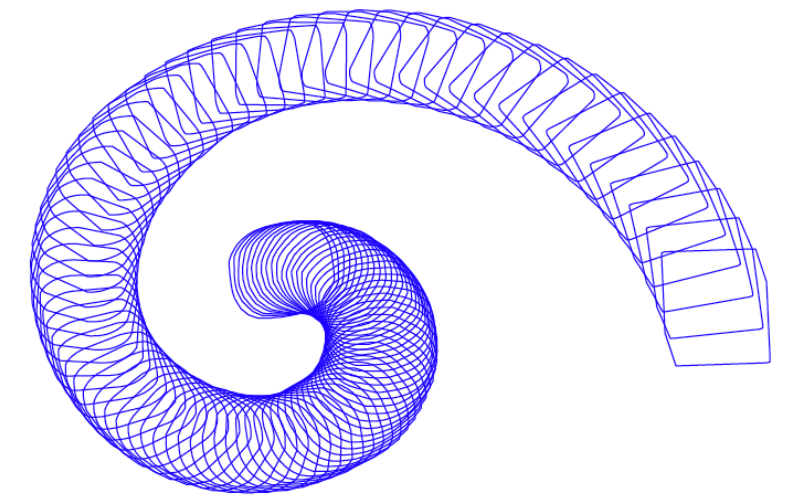
\includegraphics[width=0.5\columnwidth]{images/zono.png}
An example of a flowpipe.
\end{figure}

\end{frame}

\begin{frame}[t]{Two kind of polyhedra}
Key issue for flowpipe computation: being able to manipulate these polyhedra. There are two kind of polyhedra:
\only<2,3>{\begin{block}{$\mathcal{V}$-polyhedron}
A $\mathcal{V}$-polyhedron $P$ is the Minkowsky sum of the convex hull of a set $V$ of vertices and the conic hull of a set $C$ of vectors. $P= conv(V) + cone(C)$.
\end{block}}
\only<3>{
\begin{figure}
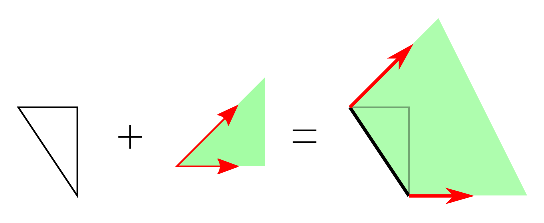
\includegraphics[scale=1]{images/vpoly.eps}\\
Construction of a $\mathcal{V}$-polytope
\end{figure}
}
\begin{itemize}
\visible<4->{\item the $\mathcal{V}$-polyhedron;}
\visible<6->{\item the $\mathcal{H}$-polyhedron.}
\end{itemize}
\only<4,5>{\begin{block}{$\mathcal{H}$-polyhedron}
An $H$-polyhedron $P$ is the intersection of a set of half-spaces: $\cap_{i=0}^n\{ x|a_i.x\leq b_i \}$. This can be written with a matrix $\{ x| Ax \leq b\}$.
\end{block}}
\only<5>{
\begin{figure}
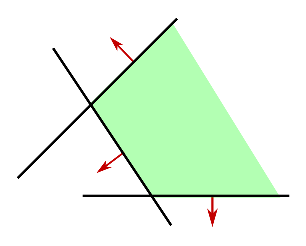
\includegraphics[scale=0.5]{images/hpoly.eps}\\
Construction of a $\mathcal{H}$-polytope
\end{figure}
}
\visible<6,7,8>{
\begin{table}
\centering
\begin{tabular}{| c | c | c | c |}
	\hline	
				    & $.\ \cap\ .$ & $.\ \cup\ .$ & $.\ +\ .$ \\ \hline
	$\mathcal{V}$-Polyhedra   & $-$ & $+$ & $+$ \\ \hline
   	$\mathcal{H}$-Polyhedra   & $+$ & $-$ & $-$\\ \hline
\end{tabular}
\caption{Comparison of the two representations.}
\end{table}
\vspace*{-0.5cm}
}

\visible<7,8>{\begin{block}{Central theorem of polyhedra representation}
A subset $P$ of $\mathbb{R}^d$ is a $\mathcal{V}$-polyhedron if and only if it is an $\mathcal{H}$-polyhedron.
\end{block}}
\visible<8>{The internship resulted in a contribution to HyPro.}
\end{frame}

\begin{frame} 
	\begin{center}{\Large Plan }\end{center}
	\tableofcontents
\end{frame}






\section{State of the art}
\label{section_sota}
Dantzig's simplex algorithm~\cite{simplex} (1947) is one of the oldest algorithms to solve linear optimization problems. Its geometric interpretation allowed the creation of a family of algorithms for the vertex enumeration problem called the pivoting algorithms~\cite{pivoting}. This section presents the required background knowledge regarding the simplex algorithm as well as one pivoting algorithm: the Avis-Fukuda algorithm~\cite{fukuda} (refereed as Fukuda's algorithm in the rest of the paper).

\subsection{The simplex algorithm}

\subsubsection{Linear optimization.}
The simplex algorithm is an algorithm that solves \emph{linear optimization problems}. A linear optimization problem is finding the maximum of a linear function (the objective) $(x_i)_{i=1}^n \mapsto \sum_{i=1}^n c_i x_i$  under a set of linear inequality constraints $\sum_{i=1}^n a_i x_i \leq b_i$. Geometrically, such a problem is to find the point which coordinates maximizes the objective, which can be seen as a direction, in an area defined by a set of half-spaces (each constraint is the equation of a half-spaces).

The set of the points respecting all the constraints is called the feasible area. To simplify the problem, the origin is assumed to be in the feasible area (equivalently: all the $b_i$ are positive) and the feasible area is assumed to be contained in $(\mathbb{R}_+)^d$. When a point is on a constraint (its coordinates turn the inequality into an equality), the constraint is called \emph{saturated}. 

The first step of the algorithm is to turn all the inequalities into equalities by the addition of positive \emph{slack} variables. These variables correspond to a distance from the associated constraint. Note that every variable (slack or not) corresponds to a constraint and thus to a half-space. Assigning a variable to a negative value means violating the corresponding constraint. In the following, the non-slack variables will be referred as \emph{original}.

\subsubsection{The dictionary.}
By adding to these equalities an other equality corresponding to the cost function, a tableau of coefficients is obtained. This tableau is called a dictionary. So far, every row corresponds to a slack variable plus one for the objective function and every column corresponds to an initial variable, plus one for the constants. In the rest of this report, the entry in the row $i$ and column $j$ is named $a_{ij}$.


The dictionary allows to find the value of every variable knowing the value of those associated to the columns. The set of the variables associated to the columns is called the \emph{cobasis}, the set of the variables associated to the row is called the \emph{basis}. Setting all the variables of the cobasis to zero provides a valuation for all the original variables. Such valuation describes a point against $d$ hyperplanes: a vertex of the hyperplane arrangement.% The cobasis is a coordinate system composed by the normal vectors of the hyperplanes associated to the variables in the cobasis, with for origin point the intersection of these hyperplanes.
In the following, the basis is called $B$, the cobasis $N$, the row corresponding to the objective function is $f$ ($\in B$) and the column containing the constants is $g$ ($\in N$).  

\subsubsection{The pivot.} 
The idea of the simplex is to exchange the variables between the basis and the cobasis (and updating in consequence the coefficients of the dictionary) such that when the cobasis is set to zero, the objective function increases and no basic variable is set to a negative value. This operation is called a pivot. From a geometrical point of view this operations consist in keeping $d-1$ constraints saturated and exchanging the remaining one for an other.%, increasing the objective and staying in the feasible area..
The vertices of the feasible area are explored until a maximum is reached. For a pivot occuring between the variables $r$ and $s$, $a_{rs}$ is refereed as the coefficient corresponding to the pivot. If it equals zero, the pivot is impossible and it means that the variable of the basis is independent from the variable from the cobasis. The most spread rule to select the pivot of a dictionary is Bland's rule~\cite{bland}, it ensures that the next dictionary describes a point in the feasible area and the termination of the algorithm.

%To maintain the fact that the cobasis expresses the vector of the basis, the following transformations are applied to the dictionary. The coefficients of the new dictionary are primed, the pivot occurs between $r \in B-f$ and $s \in N-f$ and the transformation is for all $(i,j)\in (B-r,N-s)$:
%$$ a'_{sr}=\frac{1}{a_{rs}}, \hspace{1cm} a'_{ir}=\frac{a_{is}}{a_{rs}}, \hspace{1cm} a'_{sj}=-\frac{a_{rj}}{a_{rs}}, \hspace{1cm} a'_{ij}=a_{ij}-\frac{a_{is}a_{rj}}{a_{rs}}.$$


%A major issue of the simplex is that it can loop, this is overcome with Bland's rule to pick a pivot. It ensures the termination of the algorithm and ensures the point represented by the dictionary stays inside the feasible area.

%This rules applied to the dictionary of example~\ref{lp3} calls for pivoting around the first row and the first column. Which sends $x$ to the basis and $s_1$ to the cobasis. Setting the cobasis to $0$ indicates that the dictionary represents the point $(2,0)$. The next pivoting is around the second row and the second column which leads to the point$(2,7)$, the Bland's rule then state that the optimum is reached. The example~\ref{lp4} provides the transformations of the dictionary.



\subsubsection{Some properties.}
A basic variable is primal feasible if the associated constant is non negative, a cobasic variable is said dual feasible if the associated coefficient in the objective function is non positive. A dictionary is primal (resp. dual) feasible if all the variables is the basis (resp. cobasis) are primal (resp. dual) feasible. A dictionary is optimal if it is both primal and dual feasible. A dictionary is primal feasible if and only if it describes a point inside the feasible area. A dictionary is dual feasible if and only if there is no pivot able to increase the objective.

\begin{proposition}
The normal vectors of the hyperplanes associated to the variables of the cobasis describe an independent family: the cobasis is, in fact, a basis.
\end{proposition}
\vspace*{-0.1cm}
This proposition is obtained by induction. At the beginning of the algorithm the cobasis is the canonic basis. The only operation applied to the dictionaries (the pivoting) maintain this property. If one tries to break this invariant, the new potential member of the cobasis is a linear combination of the others. This means the value of the corresponding variable is determined by the other member of cobasis which implies the pivoting provoked a division by zero.


\subsubsection{Alternative forms.}
\label{section_altsimplex}
So far, the origin is assumed to be in the feasible area and all the variables were positive. There exist alternative forms of the simplex for problems where the above assumption does not hold:

\paragraph{If the origin is not in the feasible area,} the simplex works in two phases: joining the feasible area, then optimizing. Joining the feasible area is done by an other simplex instance: 
\vspace*{-0.1cm}
\begin{itemize}
\item the constraints are the complementary half-space of each violated constraints alongside with the non violated one;
\item the function to maximize is the opposite of the sum of the slack variables corresponding to the violated constraints.
\end{itemize}
\vspace*{-0.1cm}
The simplex then continues with the initial constraints and objective function, but the current basis and cobasis.

\paragraph{If the variables are not all positive,} the idea of the simplex remains: pushing the cobasis to its bound to obtain a vertex. The sole difference is that the bounds are not $0$ anymore. Since the original variables might not be bounded, or that there might be both lower and upper bounds, a valuation for all the variables is kept (initialized at $0$ for all). The valuation is modified when a pivot occurs: the the new cobasic variable is push to its bound that maximizes the objective.


\subsubsection{An example of the simplex algorithm.} Here is given an example of use of the simplex algorithm on the linear optimization problem: maximize $x+y$ under $y\leq 2$ and $x-y\leq 2$.
\vspace*{-0.4cm}
\begin{multicols}{2}
\paragraph{Creation of the dictionary:} the slack variables are defined $0 \leq s_1 = 2-y$ and $0\leq s_2=2-x+y$. These equalities are then put together in the dictionary:
\begin{tabular}{| c | c || c || c c |}
\hline	
$x$ & $y$ & constants & & \\
$\downarrow$ &$\downarrow$ &$\downarrow$ & & \\
\hline
\hline	
$0$ & $-1$ & $2$ & = & $s_1$\\ \hline	
$-1$ & $1$ & $2$ & = & $s_2$\\ \hline \hline	
$1$ & $1$ & $0$ & $\leftarrow$ & objective function \\
\hline	
\end{tabular}

Bland's rule tells to pick $x$ and $s_2$ for the first pivot, which leads to
\begin{tabular}{| c | c || c || c c |}
\hline
$s_2$ & $y$ & const & & \\
\hline
\hline	
$0$ & $-1$ & $2$ & = & $s_1$\\ \hline	
$-1$ & $1$ & $2$ & = & $x$\\ \hline \hline	
$-1$ & $2$ & $2$ & $\leftarrow$ & obj \\
\hline	
\end{tabular}.


Then $y$ and $s_1$: 
\begin{tabular}{| c | c || c || c c |}
\hline
$s_2$ & $s_1$ & const & & \\
\hline
\hline	
$0$ & $-1$ & $2$ & = & $y$\\ \hline	
$-1$ & $-1$ & $4$ & = & $x$\\ \hline \hline	
$-1$ & $-2$ & $6$ & $\leftarrow$ & obj \\
\hline	
\end{tabular}.
There is no other pivot selected by Bland's rule, note that the final dictionary is optimal.

\columnbreak

\figurecol{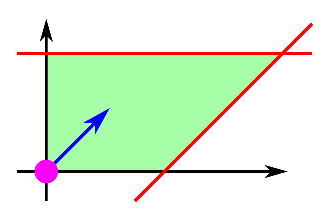
\includegraphics[width=\columnwidth]{images/simplex12.eps}%
\figcaption{Geometrical interpretation of the maximization problem. The constraints are in red, the blue arrow corresponds to the gradient of the objective function, the feasible area is shaded, the purple point is the origin (the point described by the first dictionary).}}

\figurecol{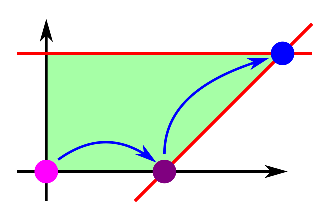
\includegraphics[width=\columnwidth]{images/simplex15.eps}%
\figcaption{The current point after the first pivot is $(2,0)$, and after the second $(4,2)$.}}



\end{multicols}























%Instead of setting the cobasis to zero, lower and/or upper bounds can be kept for each variables, alongside with a valuation (initialized at $0$ for every variable). The original variables don't have bounds. Once again the valuation of the variables of the cobasis is sufficient to determine the valuation of the basis. The dictionary stays identical (only the constants' column becomes useless). Here the variables can be positive or negative.

%The first phase will be to reach the feasible area, i.e. ensure that for all the variables, the valuation respects the bounds. To do so, let's pick a variable $i$ in the basis which bounds are not satisfied, without loss of generality let's assume the upper bound is not satisfied. Then let's pivot it with a cobasic variable $j$ smaller than its upper bound if $a_{ij}>0$ or greater than its lower bound if $a_{ij}<0$. Then the variable $i$ is assigned to its upper bound and the new valuation of the basis is computed. This operation is to be repeated until all the variables are in their bounds, a feasible point is found, or until no suitable pivot can be found, the feasible area is empty.

%The second phase, the optimization is very similar to the classic algorithm, instead of pushing the cobasis to zero, the valuation is fixed and the variables are pushed to their upper or lower bound (depending on the objective) when they are sent in the cobasis. This second phase will not be used in this paper.






\subsection{Fukuda's algorihm}

%vague overview
Fukuda's algorithm allows to enumerate all the vertices of an $\mathcal{H}$-polytope included in the positive orthant ($(\mathbb{R}_+)^d$, all its points have non-negative coordinates) for which the origin is a vertex. This algorithm uses the pivoting scheme of the simplex to explore the polytope. 

It is based on a simple idea: starting from any vertex, the simplex algorithm allows to reach a vertex maximizing a linear function by a unique (thanks to Bland's rule) path among the vertices. The algorithm picks a function maximized only by the origin on the positive orthant and walks backward on all the paths leading to it from all the vertices. Every time a vertex is encountered, it is output.

The first thing to do is to find the end of all these paths: the dictionary corresponding to the origin. It roughly consists in taking the canonical base as cobasis and the set constraints as the basis and setting $-\sum_{i=0}^d x_i$ as the cost function. All the possible pivots are tried from this dictionary. If a pivot leads to a primal feasible dictionary (defining a vertex inside the polytope) for which the Bland's method leads back to the previous point it is said to be a valid reverse Bland's pivot. It means that a step backward has been made on one of the paths, the new point is output, and the method has to be applied from this new point.

However, if a vertex is defined by more hyperplanes than required, several dictionaries will describe the same point, which is said to be degenerated. Fukuda overcomes this problem by defining a partial order on the dictionaries. This order corresponds to a lexicographic order on the basis for the dictionaries defining the same point. A point is only output if its dictionary is lexicographical minimal. Note that the algorithm continues on the dictionary, even if it is not lexicographical minimal.

If the origin is degenerated, then all the optimal dictionaries defining it have to be found. This is done by using a procedure very similar from the one above: by looking only at the hyperplanes redefining the origin, every pivot is tried. The difference is instead of using the Bland's rule, a variation of the dual Bland's rule is used. If the new dictionary is dual feasible (still an optimal for the cost function) and the dual Bland's rule brings it back to the previous one, then the new dictionary is valid with respect to the dual Bland's rule etc. This research presents the same uniqueness properties than the previous one. The previous research has to be launched from every dictionary obtained this way.

The following example illustrates Fukuda's algorithm on a polytope with no degenerated vertex:

\begin{example}
	Let $h$ be the polytope included in the positive orthant and the half-space $x+2y\leq 4$ (plus the positive orthant, i.e. $-x\leq 0$ and $-y\leq 0$) in $\mathbb{R}^2$.\\
	First step, the optimal dictionary:
	\begin{tabular}{| c | c || c || c c |}
	\hline	
	$x$ & $y$ & const & & \\
	$\downarrow$ &$\downarrow$ &$\downarrow$ & & \\
	\hline
	\hline	
   	$-1$ & $-2$ & $4$ & = & $s_1$\\ \hline \hline	
   	$-1$ & $-1$ & $0$ & $\leftarrow$ & obj \\
   	\hline	
 	\end{tabular}, 
 	$(x,s_1)$ and $(y,s_1)$ are both valid reverse Bland's pivot and gives respectively:
 	\begin{tabular}{| c | c || c || c c |}
	\hline	
	$s_1$ & $y$ & const & & \\
	$\downarrow$ &$\downarrow$ &$\downarrow$ & & \\
	\hline
	\hline	
   	$-1$ & $-2$ & $4$ & = & $x$\\ \hline \hline	
   	$1$ & $1$ & $-4$ & $\leftarrow$ & obj \\
   	\hline	
 	\end{tabular}
 	for the point $(4,0)$ and
 	\begin{tabular}{| c | c || c || c c |}
	\hline	
	$x$ & $s_1$ & const & & \\
	$\downarrow$ &$\downarrow$ &$\downarrow$ & & \\
	\hline
	\hline	
   	$-\frac{1}{2}$ & $-\frac{1}{2}$ & $2$ & = & $y$\\ \hline \hline	
   	$-\frac{1}{2}$ & $-\frac{1}{2}$ & $-2$ & $\leftarrow$ & obj \\
   	\hline	
 	\end{tabular}
 	for the point $(0,2)$. These two dictionaries have no valid reverse Bland's pivot, the enumeration is done.
	\label{example-fukuda}
\end{example}

\paragraph{Complexity:} for $n$ half-space in a space of dimension $d$, Fukuda gives a complexity of $O(nd(n+d)g)$, where $g$ is the number of vertices of the polyhedron, counted with their multiplicity (a degenerated vertex can be define in several ways, it is counted several times). 
\section{Contribution}
\label{section_contrib}
The purpose of this internship was to add two methods in HyPro: one to find the vertices, the cone and the linealty space of and $H$-polyhedron and one to find the convex hull of a $V$-polyhedron.\\
Fukuda's algorithm allows to enumerate the vertices of an $H$-polytope. The first thing to do was extending it into being able to handle non positive polytopes and then polyhedra. This method implemented, an other one had to be created to convert the convex hull problem such that he former could handle the inverse problem.
\subsection{Adaptation of Fukuda's algorithm for polyhedra}

\subsubsection{Converting to positive coordinates and detecting the linealy space}

Knowing a vertex of a polyhedron allows to find an affine transformation which sends it in the positive orthant. The process is to map the vertex to the origin and the normals of the hyperplanes defining it to the canonical base by respectively a translation and a change of basis.

Finding a vertex of the polyhedron is done using a dictionary like with the first phase of the general simplex seen in section~\ref{section_altsimplex}. In fact, obtaining a cobasis composed only by slack variables pushed to their bounds with all the other variables in their bounds gives a dictionary that describes a vertex of the polyhedron. Here the row corresponding to the cost function and the column corresponding to the constants are not used.


To do so, the first thing is to build a dictionary and to reach the feasible area, to check for emptiness. This is exactly the first phase of the simplex. Then, since the cobasis has to be composed only by slack variables, all the original variables in the cobasis are pivoted with a suitable slack variable (the corresponding coefficient has to be non null) but the assignments are not changed: it could bring the dictionary out of the polyhedron. 
\paragraph*{Detection of the linealty space:} If an original variable has no suitable slack variable to be exchanged with, it means this variable has no influence on the distance to each constrains, there is a line included in the polyhedron: a linealty space has been found. To overcome this problem, two constrains are added with opposed normal vectors, their directions being the linealty space's one, and the constant is zero for both, which might implies to reach again the feasible area once all the linealty direction are found. This provides a suitable slack variable to pivot around and the linealty space is saved, the example~\ref{ex_detect_linalty} illustrate this procedure. A cobasis full of slack variables means there exists enough independent constrains to define a vertex and there is no linealty space left.

\begin{example}
	Let's consider the following dictionary (the constrains does not matter for the linealty space detection):
	\begin{tabular}{| c | c | c | c  c |}
	\hline	
	$x$ & $y$ & $s_1$ & & \\
	$\downarrow$ & $\downarrow$ & $\downarrow$ & & \\
	\hline
	\hline	
   	$2$ & $1$ & $0$ & = & $z$ \\ \hline	
   	$0$ & $1$ & $2$ & = & $s_2$\\ \hline 
 	\end{tabular}.\\
 	The objective is to put $x$ in the cobasis, which is not possible. In fact, for any value of $x$, there is a suitable $z$ such that the current point is inside the feasible area: $z=2x$ is the equation of a linealty direction.\\
 	The constrain to add has $(1,0,2)$ as normal vector, the problem is it has to be expressed in term of $(x,y,s_1)$. The method is to add $2$ times (the coefficient corresponding to z) the value of $z$, in the end the normal vector to add is $(5,2,0)$ and the dictionary becomes:
 	\begin{tabular}{| c | c | c | c  c |}
	\hline	
	$x$ & $y$ & $s_1$ & & \\
	$\downarrow$ & $\downarrow$ & $\downarrow$ & & \\
	\hline
	\hline	
   	$2$ & $1$ & $0$ & = & $z$ \\ \hline	
   	$0$ & $1$ & $2$ & = & $s_2$\\ \hline 
   	$5$ & $2$ & $0$ & = & $s_+$\\ \hline 
   	$-5$ & $-2$ & $0$ & = & $s_-$\\ \hline 
 	\end{tabular}.
 	\label{ex_detect_linalty}
\end{example}

The last thing is pushing one by one the variables of the cobasis to their bounds. If doing so would make other variables violate their bounds, the variable is exchanged with the one which bound would be violated first, the latter is then set to its bound (note that the original variables have no bounds). A vertex is found with the hyperplanes that define it.


\subsubsection{Cone detection in Fukuda's algorithm}

Here the problem is reduced to the vertex enumeration of a potentially unbounded polyhedon in the positive orthant. Fukuda's algorithm allows to explore all the vertices. The unbounded side does not bother the algorithm: it just switches between the constrains, unboundedness is just a lack of constrain.

\begin{proposition}
Every non redundant vector of the cone lies in the intersection of $d-1$ linearly independent half-spaces which intersection with a $d_{th}$ provides a vertex of the polyhedron.
\label{prop_cone}
\end{proposition}

The proposition~\ref{prop_cone} states that to find all the vectors of the cone, it is sufficient to check every vertex for the existence of a conic direction, i.e. directions such that $n-1$ independent constrains are saturated. Fukuda's algorithm explores the polyhedron and finds all the possible arrangement of constrains that defines the vertices, thus for every definition of a vertex, the dictionary is check for the existence of a cobasic variable that can be increased while not decreasing any other (not getting closer from an other constrain) and which decreases the objective function (not getting closer from an axis). Conversely, a vector found this way is a ray included in the polyhedron: it belong to the cone. The rays can be output several times, a suppression of the duplicates is done. The example~\ref{ex_detec_cone} detects the vertices and the cones according to this procedure.

\begin{example}
	Sole constrain: $x-y\leq 2$.
	The initial dictionary:
	\begin{tabular}{| c | c || c || c c |}
	\hline	
	$x$ & $y$ & const & & \\
	$\downarrow$ & $\downarrow$ &$\downarrow$  & & \\
	\hline
	\hline		
   	$-1$ & $1$ & $2$ & = & $s_1$\\ \hline \hline	
   	$-1$ & $-1$ & $0$ & $\leftarrow$ & obj  \\
   	\hline
   	\end{tabular}. This dictionary gives $0$ as a vertex. Concerning the cones, as $s_1$ would be decreasing, $x$ does not provides a cone direction, yet $y$ does: the objective is decreased and $s_1$ increases: $(0,1)$ is a cone direction.\\
   	The next (and last) dictionary to explore is obtained by pivoting $x$ and $s_1$:
   	\begin{tabular}{| c | c || c || c c |}
	\hline	
	$s_1$ & $y$ & const & & \\
	$\downarrow$ & $\downarrow$ &$\downarrow$  & & \\
	\hline
	\hline		
   	$-1$ & $1$ & $2$ & = & $x$\\ \hline \hline	
   	$1$ & $-2$ & $-2$ & $\leftarrow$ & obj  \\
   	\hline
   	\end{tabular}
   	\label{ex_detec_cone}. The vertex obtained is $(2,0)$ and a cone direction is found: $(1,1)$ with the variable $y$.
\end{example}

The algorithm enumerates the linealty space when looking for a first vertex, and the cone and the vertices during Fukuda's algorithm: it allows to switch from an $H$-polyhedron to a $V$-polyhedron.




\subsection{From vertex enumeration to convex hull}
%define n

In geometry, vertices and half-spaces are close concepts: a vertex $(a_i)_{i=0}^d$ can be associated to an half-space $\sum_{i=0}^d x_i a_i \leq 1$ et vice-versa. This association is the \emph{geometric duality} and it allows to use the vertex enumeration algorithm to find the convex hull of a polyhedron. The emptiness and the equality to a single point of a $V$-polyhedron is trivial to check, in the following, the polyhedron and polytopes are assumed to be at least two-dimensional. 
%graphical example 
\subsubsection{The convex hull of a polytope}
The polytope studied is refereed as $P$, convex hull of the set $V$. Even it means to translate $P$, it is assumed that $\sum_{x\in V} x = 0 $. Since the polytope is at least two-dimensional, the origin is not a vertex. 

\begin{definition}[The dual of a subset of $\mathbb{R}^d$]
The dual $P^\Delta$ of a subset $P$ of $\mathbb{R}^d$ is defined by $\{c | \forall x \in P, cx\leq 1  \}$
\end{definition}

The theorem~\ref{thm_dual} holds the idea of the transformation:

\begin{theorem}
If $P$ is a polytope and $0\in P$, $P=(P^\Delta)^\Delta$.
\label{thm_dual}
\end{theorem}

Starting with the set of the vertices of $P$, the algorithm begins by switching to $P^\Delta$, which is described by a set of half-spaces. The vertices of $P^\Delta$ enumerated and the dual is taken, which leads to a set of half-spaces describing $P$. Indicing by the description mean, the algorithm does $ P_V \rightarrow P_H^\Delta \rightarrow P_V^\Delta \rightarrow P_H^{\Delta\Delta} = P_H $. 

The first step ($P_V \rightarrow P_H^\Delta$) does not hold any problem and is done with the theorem~\ref{thm_conv_dual}:
\begin{theorem}
For $P$ the convex hull of a given set $V$ of vertices, $P^\Delta=\{c | \forall x \in V, cx\leq 1\}$.
\label{thm_conv_dual}
\end{theorem}
The second step ($P_H^\Delta \rightarrow P_V^\Delta$) is done by the vertex enumeration algorithm. 

The third ($P_V^\Delta \rightarrow P_H^{\Delta\Delta}$) does not cause any problem if the origin is not on a facet of $P$ (or a face of other dimension, seen as an intersection of facets): then $P^\Delta$ is bounded and the theorem~\ref{thm_conv_dual} holds.

Otherwise, let $\{x|w.x \leq 0\}$ be a facet of $P$ (since $0$ is the iso-barycenter of $P$, $\{x| -w.x \leq 0\}$ is also a facet). Let $x\in P$, $y\in P^\Delta$ and $\alpha\in\mathbb{R}$, $(y+\alpha w).x=y.x+\alpha(w.x)=y.x$, this means that $vect(w)$ is a linealty space of $P^\Delta$. $P^\Delta=conv(V')+lineal(L')$ thus $P^{\Delta\Delta}=conv(V')^\Delta \cap L'^\bot$ by the proposition~\ref{prop_lineal_dual}. Which end the convex hull problem for a polytope.

\begin{proposition}
For $V$ a set of vertices and $L$ a set of non null vectors $(conv(V)+lineal(L))^\Delta = conv(V')^\Delta \cap L'^\bot$. 
\label{prop_lineal_dual}
\end{proposition}
\begin{proof}
Let $y\in (conv(V)+lineal(L))^\Delta$, for all $v\in V$, $l \in L$ and $\alpha\in\mathbb{R}$, $y.(v+\alpha l)\leq 1$. The inequality holding for any $\alpha$,  $y.l=0$ and $y.v\leq 1$ and $y\in conv(V')^\Delta \cap L'^\bot$. Conversely, let $y \in conv(V')^\Delta \cap L'^\bot$ which means $y.\alpha l=0$ and $y.v\leq 1$ thus $y.(v+\alpha l)\leq 1$ for all $v\in V$, $l \in L$ and $\alpha\in\mathbb{R}$: $y\in (conv(V)+lineal(L))^\Delta$.
\end{proof}

\subsubsection{The convex hull of a cone}\label{ss_conehull}
To find the convex hull of a cone $C$, the convex hull algorithm for a set of points is used.
The origin is added to the set of vectors describing the cone, as for all $c$ in $C$, the segment between the origin and $c$ must belong to the cone. Then the half-spaces for which  the constant is not zero (i.e. the origin does not saturate the constrain) are deleted. This deletion is required to ensure the unboundedness of the cone. Note that this method allows to handle a linealty direction as the sum of two vectors in the cone.

\subsubsection{The convex hull of a polyhedron}
Here the linealty space is injected in the cone (as the sum of two opposite vectors), as the treatment does not differ. Let $P=conv(V) + cone(C)$ be a polyhedron, the method is given by the following result:
\begin{proposition}
Let $P=conv(V) + cone(C)$ be a polyhedron, $C'$ the set obtained from $C$ by adding a $0$ as a $0^{th}$ coordinate to every vectors ($c \mapsto (0,c)$) and $V'$ the set obtained by, by adding a $1$ as a $0^{th}$ coordinate to every vectors ($v \mapsto (1,v)$), then $P=cone(V',C')\cap \{ x| x= (1,y), y\in \mathbb{R}^d \}$
\end{proposition}

Starting from $P$, $C'$ and $V'$ are easily obtained and $cone(V',C')$ is given in~\ref{ss_conehull}. The intersection is done as follows:
$$ \{ x\in \mathbb{R}^{d+1}| a_0x_0+\sum_{i=1}^da_ix_i\leq b\}\cap \{x|x_0=1\}=\{x\in \mathbb{R}^d|\sum_{i=1}^da_ix_i\leq b-a_0\}$$

This operation can generate half-spaces with an equation such as $0\leq b$, such half-spaces are those which does not intersect with $\{x|x_0=1\}$ and they are eliminated.






\section{Conclusion}
\begin{frame}{Conclusion}
\begin{block}{Contribution}
\begin{itemize}
\item Adaptation of Fukuda's algorithm.
\item Implementation.
\end{itemize}
\end{block}

\begin{block}{$\mathcal{H}\rightarrow\mathcal{V}$}
\begin{itemize}
\item Adapt for Fukuda. $\rightarrow$ find linealty space.
\item Fukuda's algorithm find vertices and cone directions.
\end{itemize}
\end{block}


\begin{block}{$\mathcal{V}\rightarrow\mathcal{H}$}
\begin{itemize}
\item Transform into a cone and take the geometric dual.
\item Find the vertices of the dual and take their duals to find the convex hull.
\end{itemize}
\end{block}
\end{frame}


\begin{frame}{Complexity result}
Theoretical complexity of Fukuda's algorithm: $nd(n+d)g$. $g\in \left[1;
\begin{pmatrix}
 d\\
 n 
 \end{pmatrix}\right]$

Cost of the algorithms:
\begin{itemize}
\item detect the linealty: cost of the simplex;
\item detect the cone: smaller than Fukuda's algorithm ($nd$ per vertex);
\item switch to the dual: $nd$.
\end{itemize} 

Faster than the current implementation, even in small dimension.

\end{frame}


%\begin{frame}{Going further?}

%\end{frame}

%\beginbackup
%\input{annexes.tex}
%\backupend

\end{document}

